\section{Orthogonality}
   
    \subsection{Spaces of Vectors}
        When two vectors are orthogonal they are at \(90\) degree angles to one another, which is defined as,
        \begin{equation}
            \boldsymbol{v}^T \boldsymbol{w} = 0
            \quad \textrm{and} \quad
            || \boldsymbol{v} ||^2 + || \boldsymbol{v} ||^2 = || \boldsymbol{v} + \boldsymbol{w} ||^2
        \end{equation}

        \par \hfill \break
        Subspaces may also be orthogonal, and two subspaces are said to be orthogonal if every vector of subspace \(V\)
        is orthogonal to every vector is subspace \(W\).

        \par \hfill \break
        Considering the four subspaces, that of the \textbf{row} and \textbf{column} spaces and the \textbf{nullspace} 
        and \textbf{left-nullspace}, as discussed in the previous chapter, the following relationship about their 
        orthogonality to one another can be formed, seen in the figure below,

        \begin{figure}[h]
            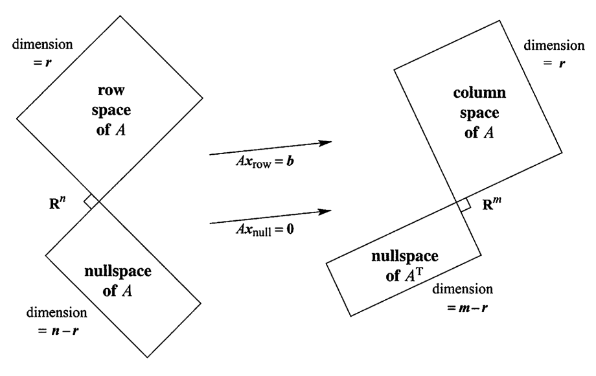
\includegraphics[width=0.75\textwidth]{the_big_picture.png}
            \centering
            \caption{The big picture}
        \end{figure}

        \par \hfill \break
        The row space of \(A\) is orthogonal (perpendicular) to the nullspace, which is all the solutions of 
        \(A\boldsymbol{x}=0\). This can be clearly seen as each row of \(A\), which make up the vectors of the row
        space, are orthogonal to each of the vectors of \(x\), which are the vectors of the nullspace.
        \begin{equation}
            A \boldsymbol{x} = 0
            \quad \textrm{expands to} \quad
            \begin{bmatrix}
                \textrm{row} \ 1 \\
                \textrm{row} \ 2 \\
                \textrm{row} \ m
            \end{bmatrix}
            \begin{bmatrix}
                \boldsymbol{x}
            \end{bmatrix}
            =
            \begin{bmatrix}
                0 \\ ... \\ 0
            \end{bmatrix}
        \end{equation}
        The column space is perpendicular (orthogonal) to the left-nullspace as every row of \(A^T\) is a column of 
        \(A\), and so as the left nullspace results in the dot product of row of \(A^T\) multiplied by the vector \(y\)
        to produce the zero vector, hence they are orthogonal.
        \begin{equation}
            A^T \boldsymbol{y} = 0
            \quad \textrm{expands to} \quad
            \begin{bmatrix}
                \textrm{row} \ 1 \\
                \textrm{row} \ 2 \\
                \textrm{row} \ m
            \end{bmatrix}
            \begin{bmatrix}
                \boldsymbol{y}
            \end{bmatrix}
            =
            \begin{bmatrix}
                0 \\ ... \\ 0
            \end{bmatrix}
        \end{equation}

        \subsubsection{Orthogonal Compliments}
            The definition of an orthogonal compliment is a subspace which contains every vector that is perpendicular
            to another subspace.

            Hence,
            \begin{itemize}
                \item The \textbf{nullspace} \(N(A)\) is the orthogonal compliment of the \textbf{row space} 
                \(C(A^T)\).
                \item The \textbf{left nullspace} \(N(A^T)\) is the orthogonal compliment of the \textbf{column space} 
                \(C(A)\).
            \end{itemize}
            This implies that a vector that is in the nullspace of a matrix \(A\) cannot therefore be in the row space,
            and conversely, a vector in the left nullspace cannot be in the column space.

        \subsubsection{Projections}
            A projection is when a vector or matrix is \textit{projected} onto a subspace of the whole space. For 
            example, starting with the vector \(b = \begin{bmatrix} 2 & 3 & 4 \end{bmatrix}\) and projecting this onto
            a line on the z-axis results in the vector \(p_1 = \begin{bmatrix} 0 & 0 & 4 \end{bmatrix}\), and 
            projecting onto the xy-plane results in the vector \(p_2 = \begin{bmatrix} 2 & 3 & 0 \end{bmatrix}\). 
            The projection matrices, which appear in the form \(\boldsymbol{p}=P\boldsymbol{b}\) are then seen as,
            \begin{equation}
                P_1 = 
                \begin{bmatrix}
                    0 & 0 & 0 \\
                    0 & 0 & 0 \\
                    0 & 0 & 1
                \end{bmatrix}
                \quad \textrm{and} \quad
                P_2 = 
                \begin{bmatrix}
                    1 & 0 & 0 \\
                    0 & 1 & 0 \\
                    0 & 0 & 0
                \end{bmatrix}
            \end{equation}
            In the case of the projections \(\boldsymbol{p}_1\) and \(\boldsymbol{p}_2\), they are perpendicular to one
            another. Each are a basis of their own subspace, and are hence \textbf{orthogonal subspaces} and \textbf{
            orthogonal compliments}. Every vector in \(b\) is the sum of its parts, such that \(\boldsymbol{p}_1 + 
            \boldsymbol{p}_2 = \boldsymbol{b}\).

            \begin{figure}[h]
                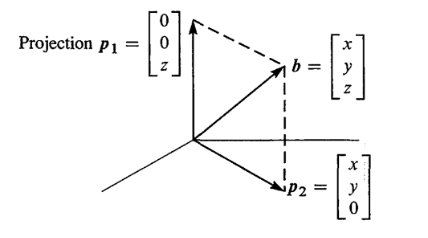
\includegraphics[width=0.5\textwidth]{projections_onto_subspace.png}
                \centering
                \caption{Projection from a vector onto a subspace}
            \end{figure}

            \par \hfill \break
            The purpose behind projections is to allow for cases when an exact solution to \(A\boldsymbol{x} = 
            \boldsymbol{b}\) cannot be found. For an exact solution to \(A\boldsymbol{x} = \boldsymbol{b}\), the vector
            \(\boldsymbol{b}\) must lie within the column space of \(A\), i.e. the matrix is square and invertible with
            full rank, etc. If \(\boldsymbol{b}\) lies outside the column space of \(A\) then a \textit{best estimate}
            solution can be found by projecting from \(\boldsymbol{b}\) onto the column space of \(A\). 

        \subsubsection{Projection Onto a Line}
            If the matrix \(A\) consists of just a single vector \(\boldsymbol{a}\), for an exact solution 
            to be found for \(A\boldsymbol{x} = \boldsymbol{b}\), then \(\boldsymbol{b}\) must lie on the line 
            \(\boldsymbol{a}\). If this is not the case, then a projection onto the line from \(\boldsymbol{b}\) can be
            found, and which is known as the \textbf{projection vector}. As the projection vector is cast onto the 
            column space of \(A\) then it is an exact solution to \(A\boldsymbol{x}\), which is written 
            \(A \boldsymbol{\hat{x}} = \boldsymbol{p}\), where \(\boldsymbol{\hat{x}}\) is the \textit{best estimate} 
            solution.

            \begin{figure}[h]
                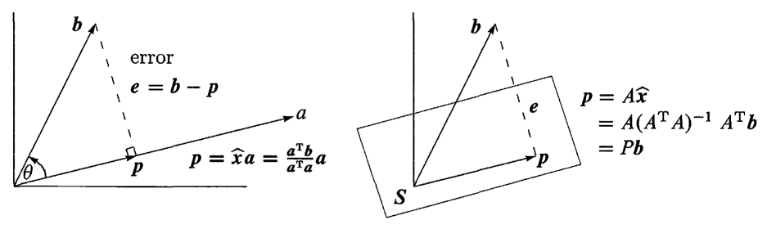
\includegraphics[width=0.750\textwidth]{projection_onto_a_line_and_space.png}
                \centering
                \caption{\textit{Best estimate} projection onto a line (\textit{left}) and space (\textit{right})}
            \end{figure}

            \par \hfill \break
            As \(A\) consists of a single line, the projection vector \(\boldsymbol{p}\) lies on \(\boldsymbol{a}\) 
            at a scaled location, i.e. \(\boldsymbol{p}=\boldsymbol{\hat{x}a}\). The projection vector 
            \(\boldsymbol{p}\) is a projection from \(\boldsymbol{b}\) onto the columns space of \(A\) at the closest 
            point, hence the vector between the two (the dotted line) is perpendicular to \(\boldsymbol{a}\), and is 
            known as the \textbf{error vector}.

            \par \hfill \break
            Using basic vector addition, \(\boldsymbol{b}=\boldsymbol{p} + \boldsymbol{e}\), hence the error vector can
            be seen as \(\boldsymbol{e}=\boldsymbol{b} - \boldsymbol{p}\). As \(\boldsymbol{p}\) can be expressed as 
            \(\boldsymbol{p}=\boldsymbol{\hat{x}a}\), then \(\boldsymbol{e} = \boldsymbol{b} - 
            \boldsymbol{\hat{x} a}\). As the error vector is orthogonal to the column space of \(A\), or simply 
            \(\boldsymbol{a}\) in this case, then \(\boldsymbol{a.e} = 0\) or alternatively \(\boldsymbol{a^T.e} = 0\). 
            Expanding this, a solution for the scale vector \(\boldsymbol{\hat{x}}\) may be found as,

            \begin{equation}
                \begin{split}
                \boldsymbol{a}^T\boldsymbol{e} = 0
                \quad \textrm{then} \quad
                \boldsymbol{a}^T (\boldsymbol{b} - \boldsymbol{\hat{x}a}) = 0
                \quad \textrm{which expands to} \quad
                \boldsymbol{a}^T \boldsymbol{b} - \boldsymbol{a}^T \boldsymbol{\hat{x}a} = 0
                \\ \\
                \boldsymbol{a}^T \boldsymbol{b} = \boldsymbol{a}^T \boldsymbol{\hat{x}a}
                \quad \textrm{and finally, as} \quad
                \boldsymbol{\hat{x}} = \dfrac{\boldsymbol{a}^T \boldsymbol{b}}{\boldsymbol{a}^T \boldsymbol{a}} 
                \end{split}
            \end{equation}

            \par \hfill \break
            Now, having found \(\boldsymbol{\hat{x}}\) the projection from \(\boldsymbol{b}\) onto the column space of 
            \(\boldsymbol{a}\) is seen as,
            \begin{equation}
                \boldsymbol{p} = 
                \boldsymbol{\hat{x}a} = \dfrac{\boldsymbol{a}^T \boldsymbol{b}}{\boldsymbol{a}^T \boldsymbol{a}} 
                \boldsymbol{a}
            \end{equation}

            \par \hfill \break
            The two special cases here are, if \(\boldsymbol{b} = \boldsymbol{a}\) then \(\boldsymbol{\hat{x}} = 1\) 
            and therefore projects onto itself, and the second being if \(\boldsymbol{b}\) is perpendicular to 
            \(\boldsymbol{a}\), resulting in \(\boldsymbol{p} = 0\).

            \par \hfill \break
            As seen in the previous section, the projection vector may be formed from a projection matrix in the form 
            \(\boldsymbol{p}=P\boldsymbol{b}\). Rearrangement of the above equation results in a projection matrix 
            being formed in the numerator, divided by a scalar, 
            \begin{equation}
                \boldsymbol{p} = \dfrac{\boldsymbol{a} \boldsymbol{a}}{\boldsymbol{a}^T \boldsymbol{a}} \boldsymbol{b}
                = P \boldsymbol{b}
                \quad \textrm{with the projection matrix being} \quad
                P = \dfrac{\boldsymbol{a} \boldsymbol{a}}{\boldsymbol{a}^T \boldsymbol{a}}
            \end{equation}

        \subsubsection{Projection Onto a Subspace}
            When \(A\) consists of multiple vectors, instead of \(\boldsymbol{b}\) projecting onto a line, \(\boldsymbol{a}\),
            it is now projecting onto a higher dimensional space. Similar to that of projection to a line, the error
            vector is perpendicular, and hence orthogonal, to every vector in \(A\).
            \begin{equation}
                A^T \boldsymbol{e} =
                \begin{bmatrix}
                    \boldsymbol{a}^T_1 \\ ... \\ \boldsymbol{a}^T_M
                \end{bmatrix}
                e = 0
            \end{equation}
            The equation may be expanded, remembering that \(\boldsymbol{e} = \boldsymbol{b} - A \boldsymbol{\hat{x}}\),
            hence,
            \begin{equation}
                A^T [\boldsymbol{b} - A \boldsymbol{\hat{x}}] = 0
                \quad \textrm{which expands to} \quad
                A^T \boldsymbol{b} - A^T A \boldsymbol{\hat{x}} = 0
                \quad \textrm{or} \quad
                A^T A \boldsymbol{\hat{x}} = A^T \boldsymbol{b}
            \end{equation}
            The best estimate solution may then be found as,
            \begin{equation}
                \boldsymbol{\hat{x}} = (A^T A)^{-1} A^T \boldsymbol{b}
            \end{equation}
            The projection vector may also be seen as,
            \begin{equation}
                \boldsymbol{p} = A \boldsymbol{\hat{x}} = A(A^T A)^{-1}A^T \boldsymbol{b}
            \end{equation}
            where the projection matrix is now,
            \begin{equation}
                P = A(A^T A)^{-1} A^T
            \end{equation}
            It should be noted that the expression \((A^T A)^{-1}\) cannot be seperated into \((A^T)^{-1}\) and 
            \(A^{-1}\), as in this case \(A \boldsymbol{x} = \boldsymbol{b}\) is not meant to have an exact solution,
            hence the mtrix \(A\) has no inverse.

        \subsection*{Least Squares Approximation}
            
        
